\documentclass[titlepage, 12pt]{article}
\usepackage{graphicx} % Required for inserting images
\usepackage{parskip}
\usepackage[left=2.5cm, right=2.5cm]{geometry}
\usepackage{graphicx}

\title{\textbf{Project Artificial Inteligence \\ Bank branches}}
\author{José Emparanza, Alberto Sainz y Santiago Norzagaray}
\date{\today}

\begin{document}

\maketitle

\tableofcontents

\newpage

\section{GitHub}
https://github.com/albertoosg/Practica-IA

\section{Description of the project}
The main objective of this project is to simulate the functioning of a bank branch, providing a realistic representation of customer service dynamics, employee roles, and operational workflow. The simulation will include multiple branches (A, B, and C), each designed to reflect the structure and organization of a real-world banking environment.

Each branch will have a designated number of service posts available to attend to customers. These posts will be responsible for handling various essential banking operations as:

- \textbf{Deposit and withdrawal of money:} Customers can deposit funds into their accounts or withdraw cash as needed.

- \textbf{Investments:} Bank employees will provide investment advice, manage financial portfolios, and assist customers in making informed investment decisions.

- \textbf{Bank loans and credits:} The bank will offer loan services, where customers can apply for personal or business loans, mortgages, and other credit-related products.

Each service post will be managed by a dedicated employee, who will be responsible for efficiently handling customer requests. In addition, each branch will have a branch manager, tasked with overseeing daily operations, ensuring workflow efficiency, and addressing any issues that arise. 

Customers will arrive at the bank branch at a and will be organized into queues based on their order of arrival. They will then be directed to the appropriate service posts based on their specific banking needs. After performing operations in the branch, the customers leave. 

Each action that happened during the simulation occurs at a specific moment in time, from the moment a customer enters the branch to the moment the customer leaves. Moreover, the simulation shows how long a customer waits in the queue until its attended by an employee in a post of the branch.

\newpage

\section{Code structure}

\subsection{Main}
Here we find the customer generator function, which creates customers during the simulation process. The random time between customer arrivals and transactions is specified, and customers are randomly assigned a counter and branch. Then the simulation environment is initialized, with the creation of as many branches as desired, with the creation of the bank, and with the generation of customers for the duration of the simulation. 

In the end, we obtain a summary of the data of each branch with which we can make a comparison of which one is more efficient, which one has more clients, or the ones that lend or receive more money for investments.

\subsection{Bank}
The Bank class serves as the central entity in the simulation, managing the overall structure and operations of the bank. It contains general information about the bank, such as its name, the total number of branches, and any additional attributes that may define its operations. This class is responsible for assigning customers to branches and ensuring a balanced distribution of clients across multiple locations.

\subsection{Clients}
The Clients class is designed to represent a customer who interacts with a bank branch in a simulated environment. This class stores and manages essential customer information while tracking their journey through the bank, from arrival to departure. Clients will be able to perform different operations, such as depositing or withdrawing money, investing, or borrowing with probability. 

Each instance of this class will hold details about an individual customer, such as their unique identification, financial status, and the type of banking operations they may require.

\subsection{Branches}
The branch class provides information on the branches and the number of counters in each branch. It has counters for the total number of customers who come to the branch, the money lent by the bank, and the money invested by the customers.

\newpage

\section{Technical Aspects}
The code simulates the activity of a multi-branch bank using the simpy library for event simulation. It is structured in four main files: main.py, which organizes the simulation; branch-client.py, which defines the clients and their operations; branch-bank.py, which handles branch assignment and summary generation; and branch.py, which stores the data for each branch.

From the design point of view, the code seeks to follow very good encapsulation practices, trying to organize the functionality in specific classes such as Client, Bank and Bank-Branch. In practice, static typing is used, which improves code clarity, and an efficient structure is used to store transactions (self.history in the Bank class). In addition, the use of the simpy library allows modeling attention queues and waiting times in a realistic way.

Performing a more technical analysis of each file, it can be observed that: 

\textbf{- main.py:} Presents a well-structured flow, since it configures branches, requests simulation parameters to the user, executes the process and generates a summary. 

\textbf{- branch-client.py:} In this class, clients execute banking operations randomly, waiting for their turn in the assigned branch. 

\textbf{- branch-bank.py:} This class manages branch randomization and generates a CSV report.

\newpage

\section{Execution analysis}

\subsection{Explanation}
By executing the project code, the program asks the user how many customers the user wants to generate to enter and operate in a branch. In addition, the program asks the user to specify the minimum and maximum amount of money that clients will have available during the simulation. Once the user answers the three requirements, the simulation starts.

These customers enter a branch at a moment in time to try to withdraw or deposit money, invest, create a bank account, manage a bank account, or request a loan. Once they perform one or more of the operations that can be performed in the branch, the customers finish their appointment in the branch.

These customers can just withdraw money if their card balance allows them to withdraw the amount of money they want. Moreover, the investment operation, in the same way that occurs with the money withdrawal, can just be carried through if the card balance allows it. As explained in the project description, the card balance allows a customer to make a money withdrawal or investment if the card balance is higher or equal to the amount of money the customer is trying to operate with.

The program shows, when running, everything that happens during the simulation. The messages that could be shown during the simulation are:

\textbf{- "Client x arrives to Bank Branch X at x time units":} This message is shown when a customer enters a branch. Specifies the number of the client, the branch it is entering, and the time at which the client has entered.

\textbf{- "Client x is being attended to at Bank Branch X at x time units. (Time waiting x time units)":} This message is shown when a customer is attended at a post by an employee. Specifies the number of the client, the branch it is in being attended to, the time at which the client has been attended to, and how long the client waited in the queue.

\textbf{- "Client x apply for a loan of x€. Current balance: x€":} This message is shown when a customer applies for a loan at a branch post. Specifies the number of the client, the amount the client applied, and the balance after performing the operation.

\textbf{- "Client x withdraw x€. Current balance: x€":} This message is shown when a customer withdraws an amount of money. Specifies the number of the client, the amount of money the customer wants to withdraw, and the balance after performing the operation (the balance must be higher than or equal to the amount invested).

\textbf{- "Client x tries to withdraw x€, but only has x€":} This message is shown when a customer tries to withdraw money, but the amount the customer wants to withdraw is not available because the card balance is not enough. Specifies the number of the client, the amount of money the customer wants to withdraw, and the balance before performing the operation (the balance must be less than the amount tried to withdraw).

\textbf{- "Client x invest x€. Current balance: x€":} This message is shown when a customer invests in a financial portfolio. Specifies the number of the client, the amount of money the customer wants to invest, and the balance after performing the operation (the balance must be higher than or equal to the amount invested).

\textbf{- "Client x cant invest x€, insufficient balance.":} This message is shown when a customer tries to invest money, but the amount the customer wants to withdraw is not available because the card balance is not enough. Specifies the number of the client, the amount of money the customer wants to invest, and the balance before performing the operation (the balance must be less than the amount tried to invest).

\textbf{- "Client x deposit x€. Current balance: x€":} This message is shown when a customer deposits an amount of money. Specifies the number of the client, the amount the customer is depositing, and the balance after performing the operation.

\textbf{- "Client x finishes his appointment at Bank Branch X at x time units":} This message is shown when a customer leaves the branch after performing one or more operations. Specifies the number of the client, the branch at which the customer has been operating, and the time at which the client has finished his appointment and leaves.

As explained in the description of the project, each operation is performed in a moment of time during the simulation, depending on when each customer has entered the branch and it is organized in the queue to be attended.

Once the simulation is finished, the program generates a summary of each branch. This summary collects all the information and every event that happened during the simulation. It shows the user the number of clients that attended each branch, the total amount of money lent by the bank in each branch, and the total amount of money invested by the clients in each branch during the simulation. 

All the information is stored at the end of the simulation in a file called "summary-branches.csv".

\newpage

\subsection{Screenshots}

\begin{figure} [h]
    \centering
    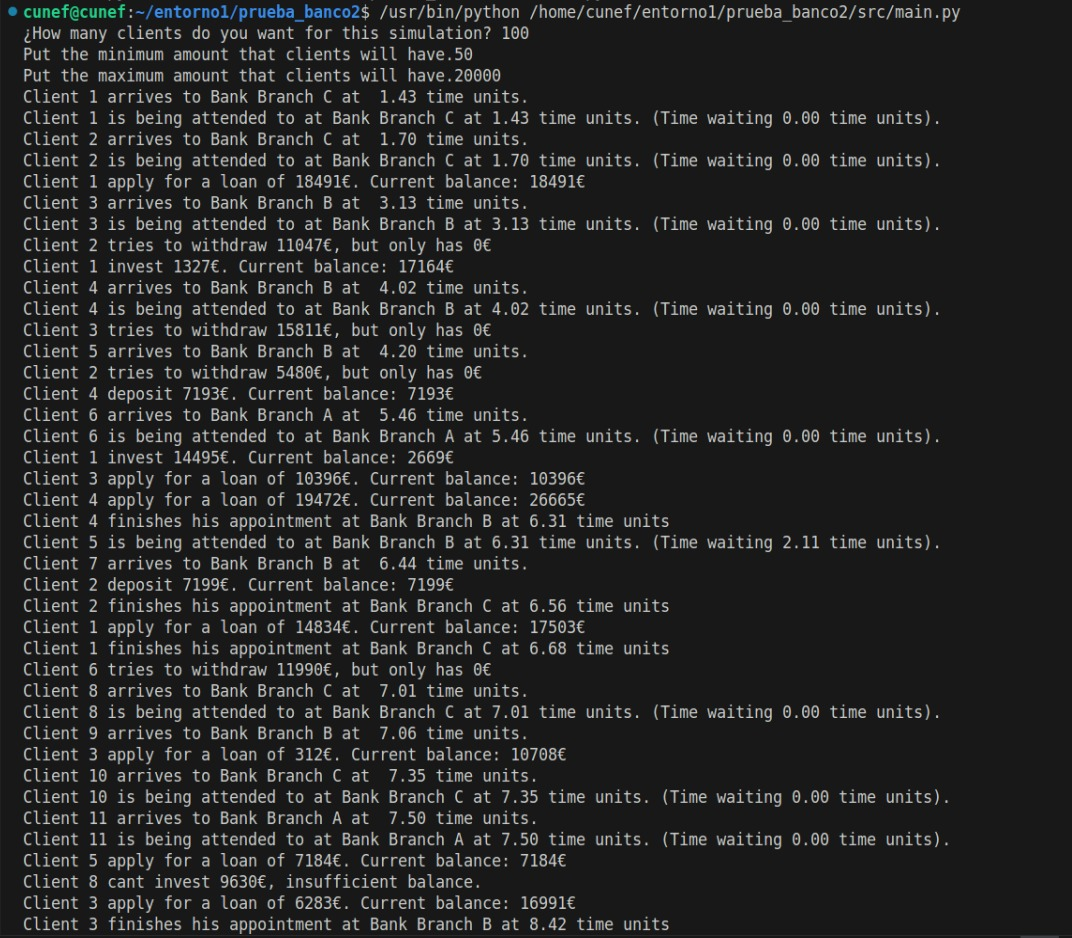
\includegraphics[scale=0.5]{Screenshots/Example Simulation 1.1.jpeg}
    \caption{Example Simulation 1.1}
    \label{fig:Example Simulation 1.1}
\end{figure}

\begin{figure} [h]
    \centering
    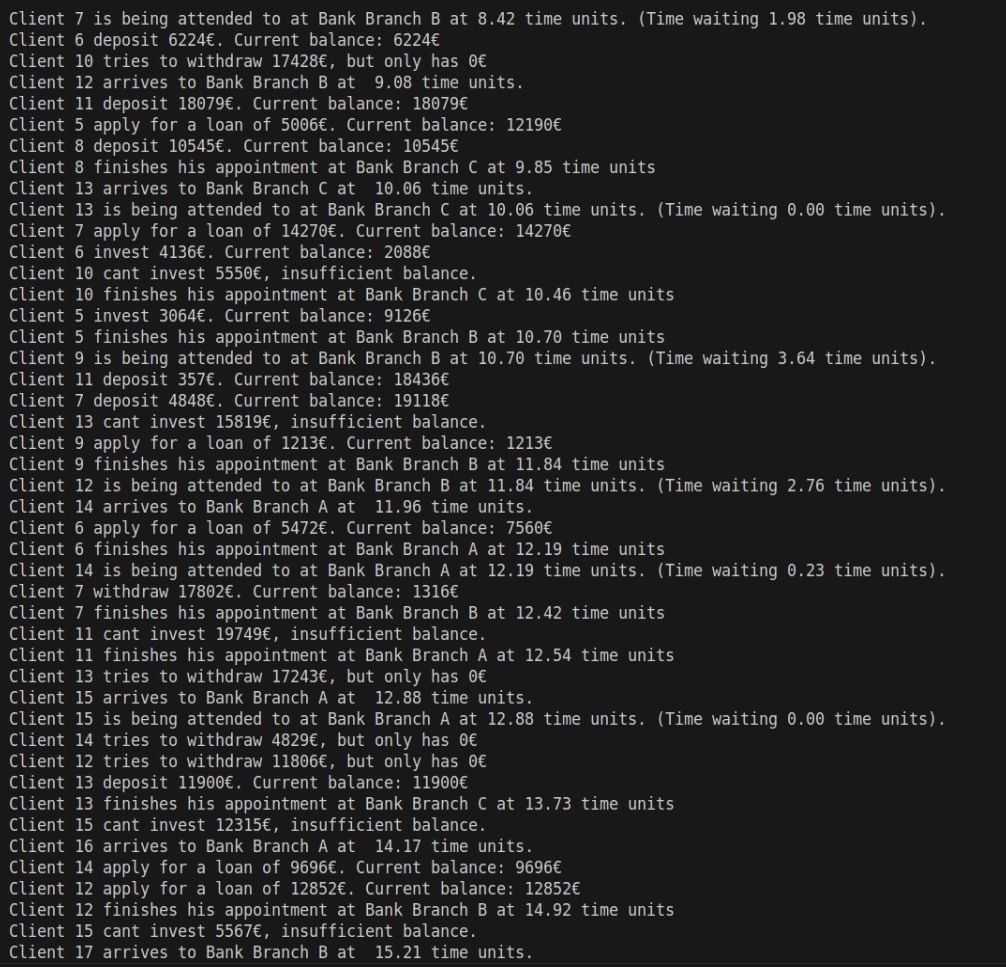
\includegraphics[scale=0.6]{Screenshots/Example Simulation 1.2.jpeg}
    \caption{Example Simulation 1.2}
    \label{fig:Example Simulation 1.2}
\end{figure}

\begin{figure} [h]
    \centering
    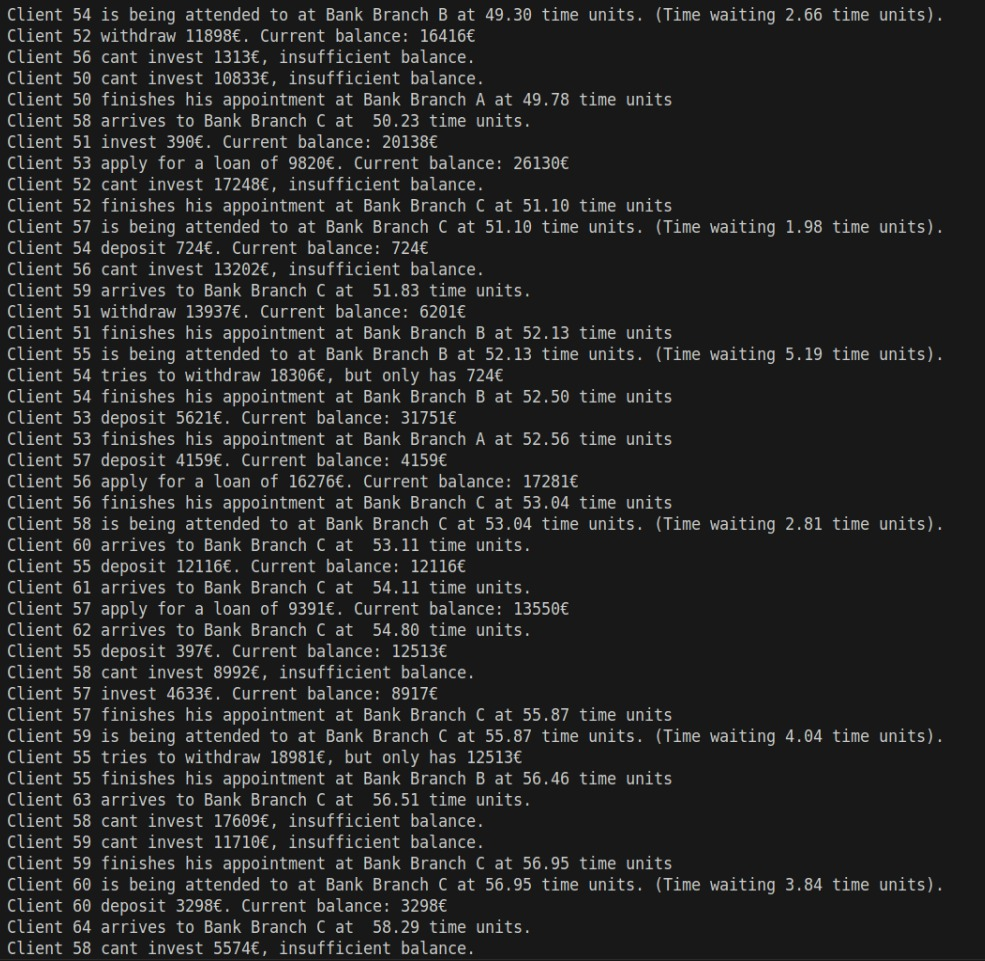
\includegraphics[scale=0.6]{Screenshots/Example Simulation 1.3.jpeg}
    \caption{Example Simulation 1.3}
    \label{fig:Example Simulation 1.3}
\end{figure}

\begin{figure} [h]
    \centering
    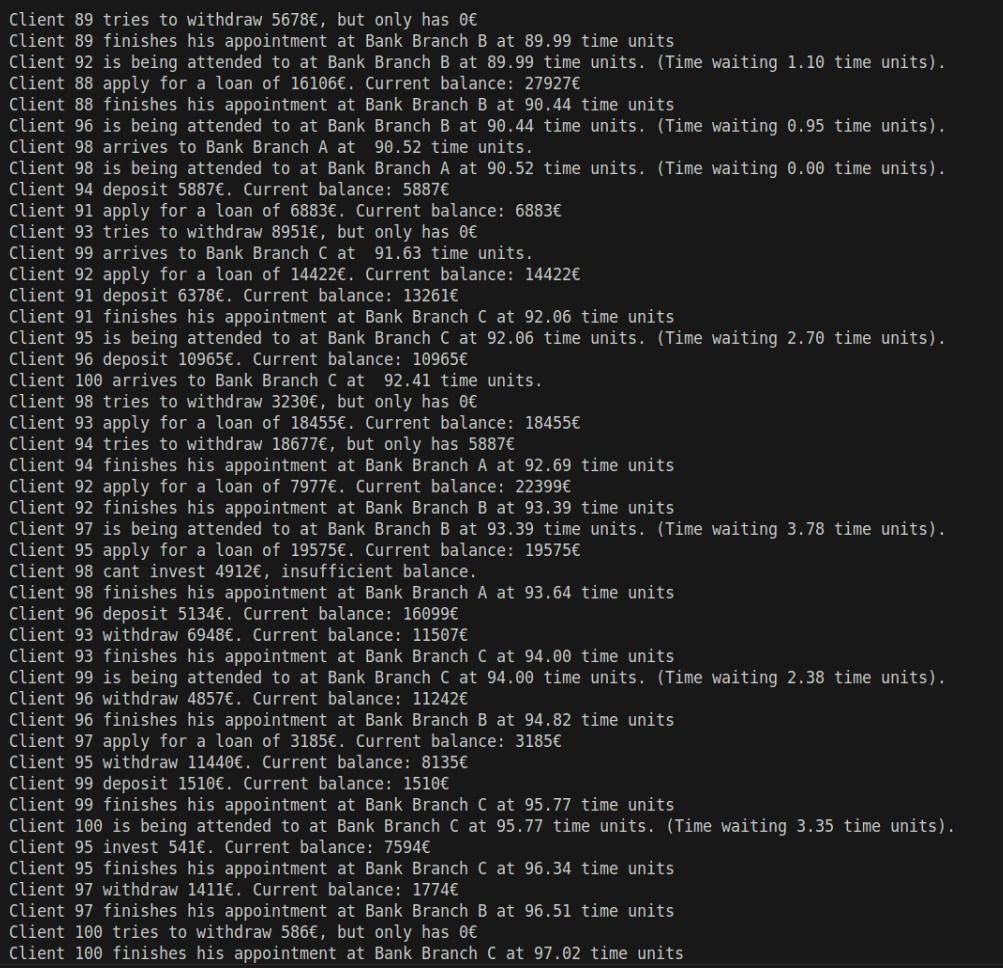
\includegraphics[scale=0.6]{Screenshots/Example Simulation 1.4.jpeg}
    \caption{Example Simulation 1.4}
    \label{fig:Example Simulation 1.4}
\end{figure}

\begin{figure} [h]
    \centering
    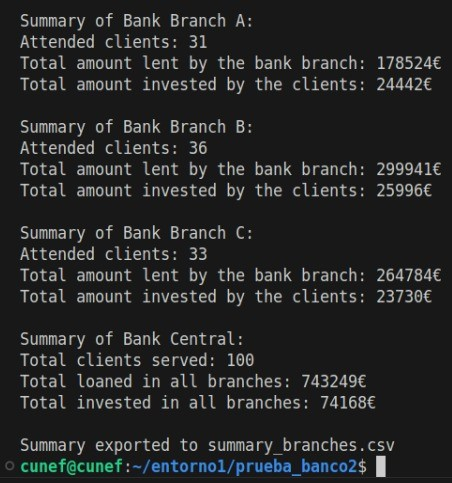
\includegraphics[scale=1]{Screenshots/Summary Simulation 1.jpeg}
    \caption{Summary Simulation 1}
    \label{fig:Summary Simulation 1}
\end{figure}

\begin{figure} [h]
    \centering
    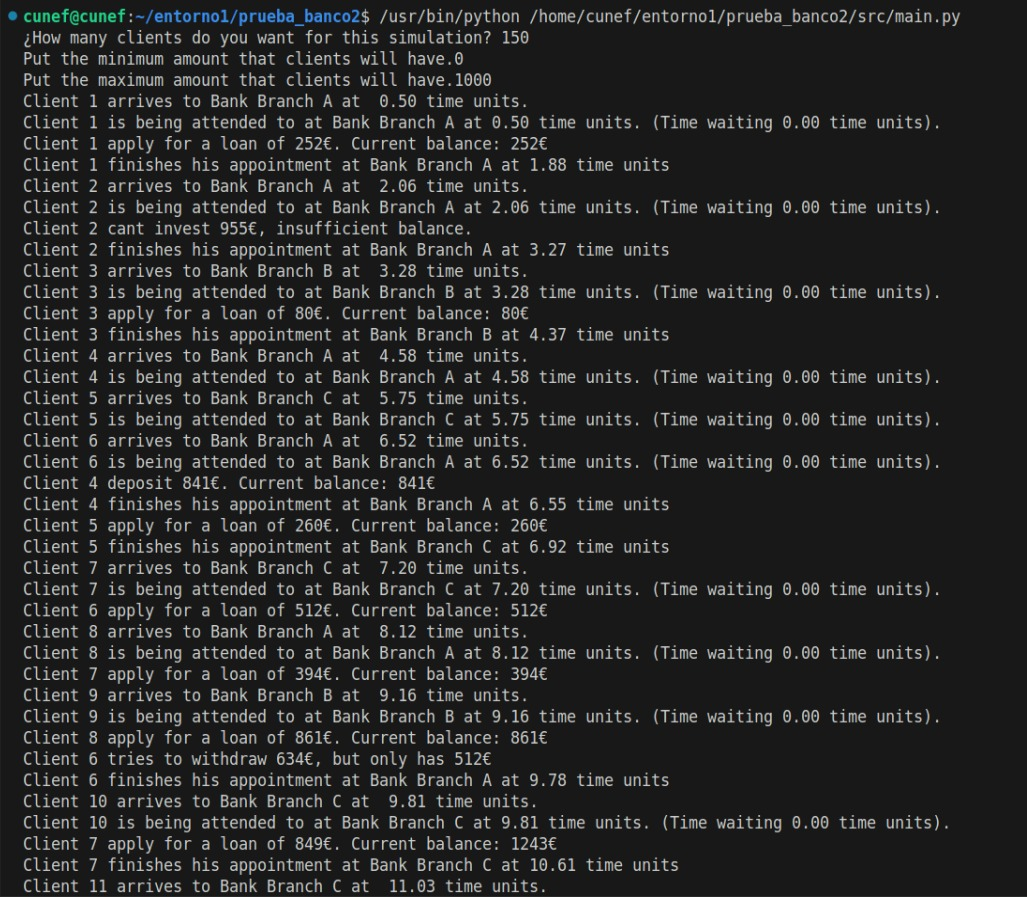
\includegraphics[scale=0.6]{Screenshots/Example Simulation 2.1.jpeg}
    \caption{Example Simulation 2.1}
    \label{fig:Example Simulation 2.1}
\end{figure}

\begin{figure} [h]
    \centering
    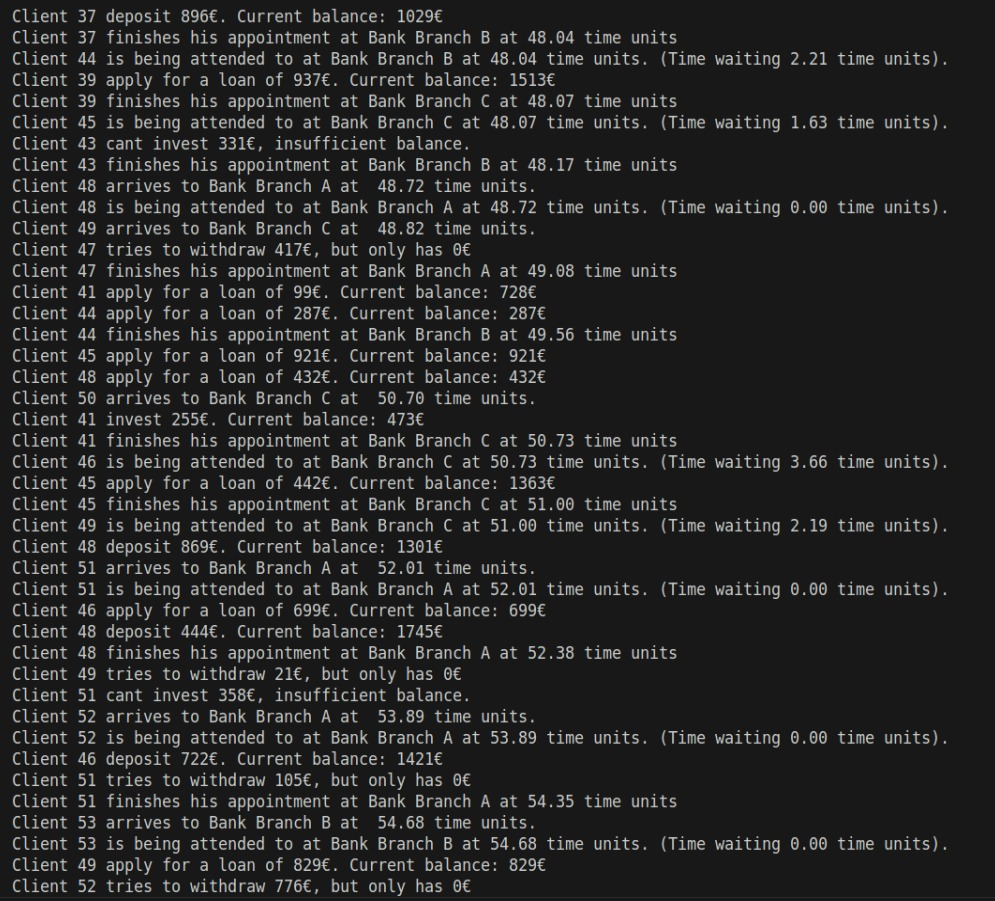
\includegraphics[scale=0.6]{Screenshots/Example Simulation 2.2.jpeg}
    \caption{Example Simulation 2.2}
    \label{fig:Example Simulation 2.2}
\end{figure}

\begin{figure} [h]
    \centering
    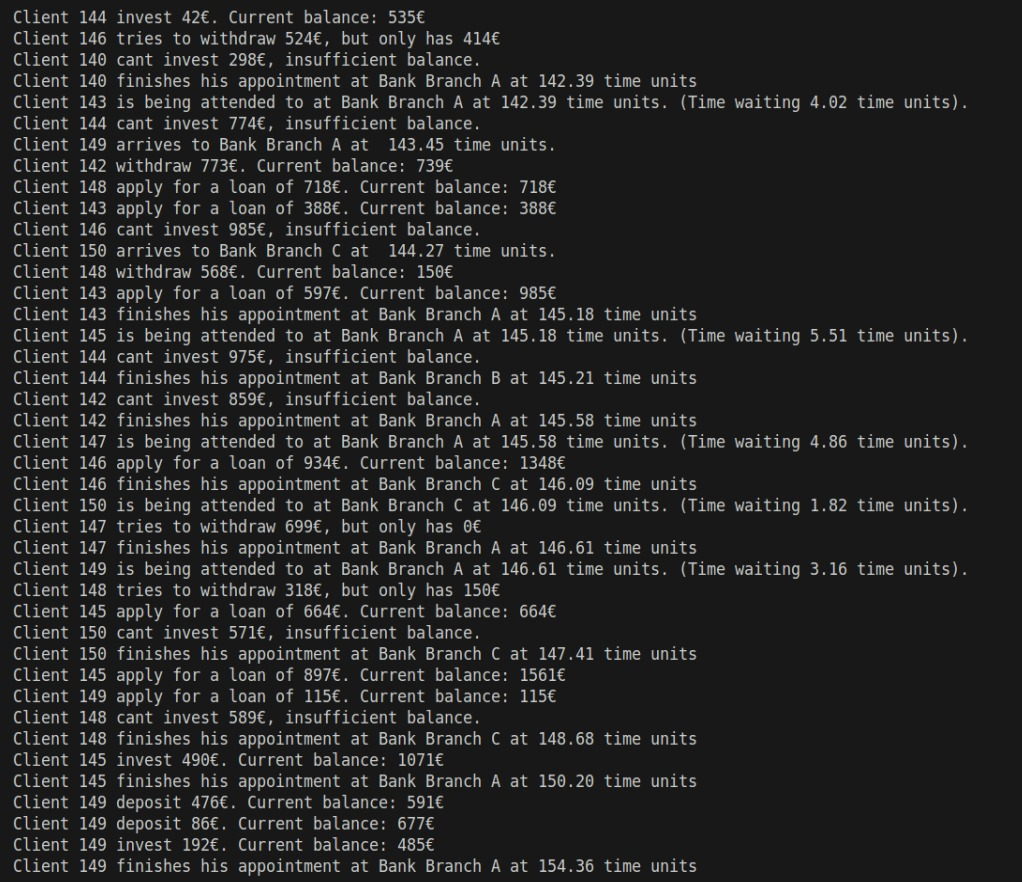
\includegraphics[scale=0.6]{Screenshots/Example Simulation 2.3.jpeg}
    \caption{Example Simulation 2.3}
    \label{fig:Example Simulation 2.3}
\end{figure}

\begin{figure} [h]
    \centering
    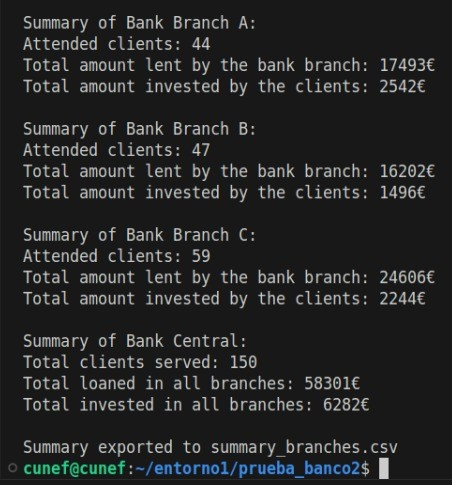
\includegraphics[scale=1]{Screenshots/Summary Simulation 2.jpeg}
    \caption{Summary Simulation 2}
    \label{fig:Summary Simulation 2}
\end{figure}

\end{document}